
\section[{\en join}]{\textgreek{Σύζευξη και είδη συζεύξεων}}

\subsection[{\en natjoin}]{\textgreek{Φυσική σύζευξη}}

\begin{frame}[t, fragile, shrink]
\frametitle{Η σχεσιακή πράξη της φυσικής σύζευξης}
\begin{minipage}{\wE}
  \begin{block}{Ορισμός της φυσικής σύζευξης} 
    \[
       \begin{split}
       r \bowtie s = \{ t \,|\, \text{ υπάρχουν πλειάδες } \, u \in r \text{ και } v \in s   \\
                \text{ έτσι ώστε } t[R]=u \text{ και } t[S]=v\}         
       \end{split}
    \]
    \par Αν η $r$ είναι σχέση με σχήμα $R=\{X,Y\}$ και $s$ είναι σχέση με σχήμα $S=\{Y,Z\}$,
    τότε η {\bf φυσική σύζευξη} των $r$ και $s$
    είναι μια σχέση με σχήμα $R \cup S = \{X,Y,Z\}$ και κορμό το σύνολο των συνδυασμών των
    πλειάδων της $r$ και $s$ για τις οποίες οι τιμές στο κοινό γνώρισμα $Y$ ταυτίζονται.   \\
    Η φυσική σύζευξη των σχέσεων $r$ και $s$ συμβολίζεται με $r \bowtie s$,
    ή $r \, \mathrm{NATURAL\, JOIN} \, s$, ή απλά $r \, \mathrm{JOIN} \, s$.
  \end{block}
\end{minipage}
\end{frame}



\begin{frame}[t, fragile, shrink]
\frametitle{Παράδειγμα φυσικής σύζευξης}
  \scalebox{1.5}{ \en
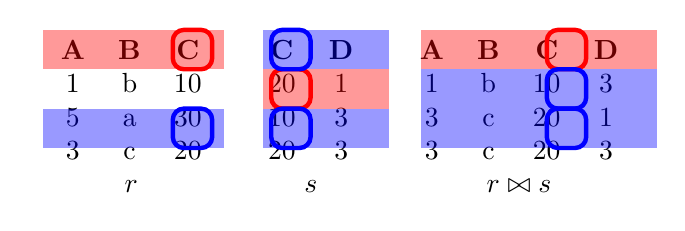
\begin{tikzpicture}

\node[anchor=south west,inner sep=0] at (0,0)
{
\begin{tabular}{ c c c }
  \begin{tabular}{ c c c }    \toprule
    {\bf A} & {\bf B} & {\bf C}  \\             \midrule
    1 & b & 10 \\
    5 & a & 30 \\
    3 & c & 20 \\             \bottomrule
  \end{tabular}
&
  \begin{tabular}{ c c }      \toprule
    {\bf C} & {\bf D}   \\                \midrule
    20 & 1  \\
    10 & 3  \\
    20 & 3  \\                \bottomrule
  \end{tabular}
&
  \begin{tabular}{ c c c c }  \toprule
    {\bf A} & {\bf B} & {\bf C}  & {\bf D}  \\        \midrule
    1 & b & 10 & 3  \\
    3 & c & 20 & 1  \\
    3 & c & 20 & 3  \\        \bottomrule
  \end{tabular}
\\
  $r$ & $s$ & $r \bowtie s$ \\
\end{tabular}  
} ;


% red 10
\pause
\draw[red,ultra thick,rounded corners] (1.85,1.7) rectangle node[above] {} + (0.5,0.5);
\draw[red,ultra thick,rounded corners] (3.10,1.2) rectangle node[above] {} + (0.5,0.5);

% red rows
\pause
\draw[red,ultra thick,rounded corners] (6.60,1.7) rectangle node[above] {} + (0.5,0.5);
\fill[red, opacity=0.4]      (0.20,1.7) rectangle node[above] {} + (2.3,0.5);
\fill[red, opacity=0.4]      (3.00,1.2) rectangle node[above] {} + (1.6,0.5);
\fill[red, opacity=0.4]      (5.00,1.7) rectangle node[above] {} + (3.0,0.5);

% blue 20
\pause
\draw[blue,ultra thick,rounded corners] (1.85,0.7) rectangle node[above] {} + (0.5,0.5);
\draw[blue,ultra thick,rounded corners] (3.10,1.7) rectangle node[above] {} + (0.5,0.5);
\draw[blue,ultra thick,rounded corners] (3.10,0.7) rectangle node[above] {} + (0.5,0.5);

%blue rows 
\pause
\draw[blue,ultra thick,rounded corners] (6.60,1.2) rectangle node[above] {} + (0.5,0.5);
\draw[blue,ultra thick,rounded corners] (6.60,0.7) rectangle node[above] {} + (0.5,0.5);
\fill[blue, opacity=0.4]      (0.20,0.7) rectangle node[above] {} + (2.3,0.5);
\fill[blue, opacity=0.4]      (3.00,1.7) rectangle node[above] {} + (1.6,0.5);
\fill[blue, opacity=0.4]      (3.00,0.7) rectangle node[above] {} + (1.6,0.5);
\fill[blue, opacity=0.4]      (5.00,1.2) rectangle node[above] {} + (3.0,0.5);
\fill[blue, opacity=0.4]      (5.00,0.7) rectangle node[above] {} + (3.0,0.5);


\end{tikzpicture}
\el  } 
  \begin{minipage}{\wE} 
    \begin{block}{Παρατηρήσεις}
      \begin{enumerate}
        \item Τα κοινά γνωρίσματα, εδώ το {\en\em C}, μόνο μία φορά στο αποτέλεσμα.
        \item Πλειάδες με μη ταιριαστές τιμές δεν συμμετέχουν στο αποτέλεσμα.
      \end{enumerate}
  \end{block}
\end{minipage}
\end{frame}

\begin{frame}[t, fragile, shrink]
\frametitle{Υπάλληλοι και τμήματα, ξένο κλειδί, 1:Ν}
\small
%\begin{minipage}{\wE}
  \begin{tabular} { l  l }
    \shortstack{
    {\bb\en departments}: \\ 
    \begin{tabular}{ c l } \toprule
    {\en\bf depid} & {\en\bf depname} \\ \midrule
    1 & Μελετών \\
    2 & Λογιστήριο \\
    3 & Διαφήμισης \\ \bottomrule
      & \\
      & \\ 
    \end{tabular}
    }
    &
    \shortstack{
    {\bb\en employees}: \\  
    \begin{tabular}{ c l c } \toprule
      {\en\bf empid} & {\en\bf empname} & {\en\bf depid} \\ \midrule
      102 & Αποστολάκης & 2 \\
      154 & Βασιλάκης   & 1 \\
      132 & Χρηστάκης   & 2\\ 
      432 & Δημητράκης  & 3 \\
      203 & Κωστάκης    & 1 \\ \bottomrule
    \end{tabular}
    }
  \end{tabular}
  \par
  %\bigskip
  {\bb\en departments $\bowtie$ employees}: \\
  \begin{tabular}{ c l c l } \toprule
    {\en\bf depid} & {\en\bf depname} & {\en\bf empid} & {\en\bf empname} \\ \midrule
    1 & Μελετών & 154 & Βασιλάκης  \\
    1 & Μελετών & 203 & Κωστάκης   \\
    2 & Λογιστήριο & 102 & Αποστολάκης \\
    2 & Λογιστήριο & 132 & Χρηστάκης \\
    3 & Διαφήμισης & 432 & Δημητράκης \\ \bottomrule
  \end{tabular} 

%\end{minipage}
\end{frame}


\subsection[{\en theta}]{\textgreek{Θήτα σύζευξη}}


\begin{frame}[t, fragile, shrink]
\frametitle{Η σχεσιακή πράξη της σύζευξης θ}
\begin{minipage}{\wE}
  \begin{block}{Ορισμός}
    \par Αν η $r$ είναι σχέση με σχήμα $R=\{A_1, A_2, \ldots, A_n\}$,
    $s$ είναι σχέση
    με σχήμα $S=\{B_1, B_2, \ldots, B_m\}$,
    τα γνωρίσματα $A_i$ και $B_j$ έχουν το ίδιο πεδίο ορισμού,
    και $\theta$ είναι τελεστής σύγκρισης, $\theta \in \{=,\neq,<,\leq,>,\geq\}$, 
    \par τότε η $\theta$ σύζευξη των $r$ και $s$, $r \bowtie_{A_i \theta B_j} s$,
    \par είναι μια σχέση με σχήμα
    το σύνολο των γνωρισμάτων των $R$ και $S$, $\{A_1, A_2, \ldots, A_n\, B_1, B_2, \ldots, B_m\}$
    και κορμό το σύνολο των πλειάδων από κάθε συνδυασμό των πλειάδων των $r$ και $s$,
    που ικανοποιούν τη συνθήκη $A_i \theta B_j$.
  \end{block}
\end{minipage}
\end{frame}



\begin{frame}[t, fragile, shrink]
\frametitle{Παρατηρήσεις για τη θ σύζευξη}
\begin{minipage}{\wE}
  \begin{itemize}   \itemsep6pt
    \item Το αποτέλεσμα είναι μια σχέση με βαθμό $n_R+n_S$,
          και πληθικότητα ανάμεσα στο 0 και στο $m_r \cdot m_s$.
    \item Αν κάποια πλειάδα έχει στο γνώρισμα που συμμετέχει
          στη σύζευξη  τιμή {\sq NULL} τότε δεν συμμετέχει στο αποτέλεσμα.
    \item Αν ο τελεστής $\theta$ είναι το $=$ τότε η σύζευξη καλείται {\bb ισοσύζευξη}.
    \item Η σύζευξη $\theta$ ($\theta\, \mathrm{JOIN}$) είναι παράγωγη πράξη γινομένου και επιλογής,
          έτσι ισχύει: \\
          {\Large \[ \sigma_{X \theta Y}(r \times s) = r \bowtie_{X \theta Y} s \]  }
  \end{itemize}
\end{minipage}
\end{frame}



\begin{frame}[t, fragile, shrink]
\frametitle{Παράδειγμα  σύζευξης θ, ξένο κλειδί, 1:Ν }
  \vspace{-1em}
  \begin{columns}[T]
    \begin{column}{0.5\textwidth}
    {\bb\en departments}:\\
    \begin{tabular}{c l} \toprule
      {\en\bf depcode} & {\en\bf depname} \\ \midrule
      1 & Μελετών \\
      2 & Λογιστήριο \\
      3 & Διαφήμισης \\ \bottomrule
    \end{tabular}
    \end{column}
    \begin{column}{0.5\textwidth}
    {\bb\en employees}: \\
    \begin{tabular}{c l c} \toprule
      {\en\bf empid} & {\en\bf empname} & {\en\bf depid} \\ \midrule
      102 & Αποστολάκης & 2 \\
      154 & Βασιλάκης   & 1 \\
      132 & Χρηστάκης   & 2\\
      432 & Δημητράκης  & 3 \\
      203 & Κωστάκης    & 1 \\ \bottomrule
    \end{tabular} 
    \end{column}
  \end{columns}
  \par
  \bigskip
  {\bb\en departments $\bowtie_{depcode=depid}$ employees}: \\
  \begin{tabular}{c l c l c} \toprule
    {\en\bf depcode} & {\en\bf depname} & {\en\bf empid} & {\en\bf empname} & {\en\bf depid} \\ \midrule
    1 & Μελετών & 154 & Βασιλάκης  & 1\\
    1 & Μελετών & 203 & Κωστάκης   & 1\\
    2 & Λογιστήριο & 102 & Αποστολάκης & 2\\
    2 & Λογιστήριο & 132 & Χρηστάκης  & 2\\
    3 & Διαφήμισης & 432 & Δημητράκης & 3\\ \\bottomrule
  \end{tabular}
\end{frame}



\begin{frame}[t, fragile, shrink]
\frametitle{Ενδυματολογικές προτιμήσεις και θ σύζευξη}
\begin{minipage}{\wE}
  %\begin{block}{Παπούτσια και Φούστες}
    \en
    \begin{columns}[T]
      \begin{column}{0.5\textwidth}
        {\bb\en shoes:} \\
        \begin{tabular}{l c}  \toprule
          {\en\bf color} & {\en\bf price} \\     \midrule
          blue  & 55 \\
          green & 45 \\
          red   & 30 \\ \bottomrule
                &    \\
        \end{tabular}
      \end{column}
      \begin{column}{0.5\textwidth}
        {\bb\en skirts:} \\
        \begin{tabular}{l c}  \toprule
          {\en\bf color} & {\en\bf price} \\     \midrule
          red     & 30 \\
          green   & 40 \\
          green   & 65 \\
          blue    & 30 \\ \bottomrule
        \end{tabular}
      \end{column}
    \end{columns}
    \el
  %\end{block}
  \begin{block}{Να βρεθούν οι συνδυασμοί:}
    \begin{enumerate}  \itemsep9pt
      \item Παπούτσια και φούστες ίδιου χρώματος.
      \item Παπούτσια και φούστες διαφορετικού χρώματος.
      \item Παπούτσια και φούστες με ακριβότερη τη φούστα.
    \end{enumerate}
  \end{block}
\end{minipage}
\end{frame}


\begin{frame}[t, fragile, shrink]
\frametitle{Παπούτσια και φούστες ίδιου χρώματος}
\begin{minipage}{\wE}
  {\Large \[ shoes \bowtie_{shoes.color=skirts.color} skirts \]  }
  \par
  \en
  \begin{tabular}{l c l c}  \toprule
    {\en\bf shoes.color} & {\en\bf shoes.price} & {\en\bf skirts.color} & {\en\bf skirts.price}\\     \midrule
       blue  & 55 & blue & 30 \\
       green & 45 & green & 40 \\
       green & 45 & green & 65 \\
       red   & 30 & red & 30 \\ \bottomrule
  \end{tabular}
\end{minipage}
\end{frame}


\begin{frame}[t, fragile, shrink]
\frametitle{Παπούτσια και φούστες διαφορετικού χρώματος}
\begin{minipage}{\wE}
  {\Large \[ shoes \bowtie_{shoes.color \neq skirts.color} skirts \]  }
  \par
  \en
  \begin{tabular}{l c l c}  \toprule
    {\en\bf shoes.color} & {\en\bf shoes.price} & {\en\bf skirts.color} & {\en\bf skirts.price}\\     \midrule
       blue  & 55 & red   & 30 \\
       blue  & 55 & green & 40 \\
       blue  & 55 & green & 65 \\
       green & 45 & red   & 30 \\
       green & 45 & blue  & 30 \\
       red   & 30 & green & 40 \\
       red   & 30 & green & 65 \\
       red   & 30 & blue  & 30 \\ \bottomrule
  \end{tabular}
\end{minipage}
\end{frame}


\begin{frame}[t, fragile, shrink]
\frametitle{Παπούτσια και φούστες με ακριβότερη φούστα}
\begin{minipage}{\wE}
  {\Large \[ shoes \bowtie_{shoes.price < skirts.price} skirts \]  }
  \par
  \en
  \begin{tabular}{l c l c}  \toprule
    {\en\bf shoes.color} & {\en\bf shoes.price} & {\en\bf skirts.color} & {\en\bf skirts.price}\\     \midrule
       blue  & 55 & green & 65 \\
       green & 45 & green & 65 \\
       red   & 30 & green & 40 \\
       red   & 30 & green & 65 \\ \bottomrule
  \end{tabular}
\end{minipage}
\end{frame}


\subsection[{\en outerjoin}]{\textgreek{Εξωτερική σύζευξη}}


\begin{frame}[t, fragile, shrink]
\frametitle{Eξωτερική σύζευξη}
\begin{minipage}{\wE}
\begin{block}{Ορισμός εξωτερική σύζευξης}
  Αν η $r$ είναι σχέση με σχήμα $R= \{ X, Y \} $,
  $s$ είναι σχέση με σχήμα $S=\{Y, Z\}$,
  τότε η εξωτερική σύζευξη
  $t = r \ojoin s$ έχει σχήμα $T=\{X,Y,Z\}$ και κορμό που
  αποτελείται από : 
  \vspace{0.5cm}
  \begin{enumerate} \itemsep 6pt
    \item Τις πλειάδες της εσωτερικής σύζευξης  των $r \bowtie s$
    \item Τις πλειάδες της σχέσης $r$ που δεν έχουν ταιριαστές τιμές στην $s$,
          με τιμές {\sq NULL} στα αντίστοιχα γνωρίσματα της $s$
    \item Τις πλειάδες της σχέσης $s$ που δεν έχουν ταιριαστές τιμές στην $r$,
          με τιμές {\sq NULL} στα αντίστοιχα γνωρίσματα της $r$
  \end{enumerate}
\end{block}
\end{minipage}
\end{frame}


\begin{frame}[t, fragile, shrink]
\frametitle{Εξωτερική σύζευξη}
  \begin{block}{Επέκταση της σύζευξης}
    Η εξωτερική σύζευξη είναι επέκταση της σύζευξης, στην περίπτωση που υπάρχουν πλειάδες σε μία
    ή περισσότερες σχέσεις, χωρίς ταιριαστές τιμές. 
  \end{block}
  \begin{exampleblock}{Για παράδειγμα:}
    \par θεωρείστε τις δύο σχέσεις του σχήματος,
    που παριστάνουν ένα δείγμα από τα υποκαταστήματα (Υ) και τους πελάτες (Π)
    μιας εταιρείας.  
    \par Θέλουμε να βρούμε το αποτέλεσμα της εξωτερικής σύζευξης
    των δύο σχέσεων με βάση την πόλη:
    \[ \Upsilon \quad \ojoin \quad \Pi \]
    Δηλαδή τα υποκαταστήματα, ανεξάρτητα από το αν έχουν ή όχι πελάτες,
    και τους πελάτες, ανεξάρτητα από το αν υπάρχει υποκατάστημα στην πόλη τους.
  \end{exampleblock}
\end{frame}



\begin{frame}[t, fragile, shrink]
\frametitle{Εξωτερική σύζευξη}
  \begin{columns}[T]
    \begin{column}{0.5\textwidth}
      {\bb Υ}\\
      \begin{tabular}{ c l } \toprule
          {\en\bf id} & {\en\bf city} \\ \midrule
          1 & Αθήνα \\ 
          2 & Πάτρα \\ 
          3 & Θεσσαλονίκη \\ \bottomrule
      \end{tabular}
    \end{column}
    \begin{column}{0.5\textwidth}
    {\bb Π}\\
    \begin{tabular}{ l l } \toprule
      {\en\bf name} & {\en\bf city} \\ \midrule
          Νίκος & Πάτρα \\ 
          Βάσω  & Κοζάνη \\ 
          Αγγελική & Πάτρα \\ 
          Βασίλης & Αθήνα \\ \bottomrule
      \end{tabular} 
    \end{column}
  \end{columns}
  \bigskip
  {\bb Υ $\ojoin$ Π}   \\
  \begin{tabular}{c l l l} \toprule
      {\en\bf id} & {\en\bf city} & {\en\bf name}  \\ \midrule
      1 & Αθήνα & Βασίλης   \\ 
      2 & Πάτρα & Νίκος    \\ 
      2 & Πάτρα & Αγγελική  \\ 
      3 & Θεσσαλονίκη & {\sq NULL}   \\
      {\sq NULL} & Κοζάνη & Βάσω   \\ \bottomrule
  \end{tabular}
\end{frame}



\subsection[{\en leftjoin}]{\textgreek{Αριστερή εξωτερική σύζευξη}}

\begin{frame}[t, fragile, shrink]
\frametitle{Αριστερή εξωτερική σύζευξη}
\begin{minipage}{\wE}
  \begin{block}{Ορισμός}
    Αν $r$ είναι σχέση με σχήμα $R=\{X,Y\}$
    και $s$ είναι μία σχέση
    με σχήμα $S=\{Y,Z\}$, τότε η αριστερή εξωτερική σύζευξη
    $t = r \lojoin s$ έχει σχήμα $T=\{X,Y,Z\}$ και κορμό
    που αποτελείται από τις πλειάδες:
    \[
       r \lojoin s = (r \bowtie s) \cup \left((r - \Pi_R (r \bowtie s)\right) \times w )
    \]
    όπου $w$ είναι μία σχέση με σχήμα $R-S$ και μία πλειάδα με τιμές $\{null, null, \ldots, null\}$.
  \end{block}
\end{minipage}
\end{frame}


\begin{frame}[t, fragile, shrink]
\frametitle{Δηλαδή}
\begin{minipage}{\wE}
  \begin{block}{Επεξήγηση ορισμού αριστερής σύζευξης}
     Η {\bf αριστερή εξωτερική σύζευξη} (ή απλώς αριστερή σύζευξη):
     \[  r \lojoin s  \]
     έχει σαν αποτέλεσμα μια σχέση με:

    \begin{itemize}
      \item Σχήμα όμοιο αυτό της φυσικής σύζευξης $r \bowtie s$.
      \item Κορμό τις πλειάδες που προκύπτουν από την ένωση των πλειάδων:
      \begin{itemize}
        \item της φυσικής σύζευξης $r \bowtie s$
        \item όλων των πλειάδων της $r$ (αριστερής σχέσης) που δεν είναι
              στο αποτέλεσμα της φυσικής σύζευξης,
              με \tnull\ τιμές στα γνωρίσματα της $s$ (δεξιάς σχέσης)
      \end{itemize}
    \end{itemize} 
  \end{block}
\end{minipage}
\end{frame}



\begin{frame}[t, fragile, shrink]
\frametitle{Παράδειγμα αριστερής σύζευξης}
\begin{minipage}{\wE}
   \begin{tabular}{l l}
     {\bb Υ} & {\bb Π} \\
     \begin{tabular}{ c l } \toprule
       {\en\bf id} & {\en\bf city} \\ \midrule
       1 & Αθήνα \\
       2 & Πάτρα \\
       3 & Θεσσαλονίκη \\ \bottomrule
         & \\
     \end{tabular} \quad
     &
     \begin{tabular}{ l l } \toprule
       {\en\bf name} & {\en\bf city} \\ \midrule
       Νίκος & Πάτρα \\
       Βάσω  & Κοζάνη \\
       Αγγελική & Πάτρα \\
       Βασίλης & Αθήνα \\ \bottomrule
     \end{tabular}
     \\
     &               \\
    {\bb  Υ $\lojoin$ Π} & {\bb  Υ $\bowtie$ Π}\\                         
    \begin{tabular}{ c l l } \toprule
      {\en\bf id} & {\en\bf city} & {\en\bf name} \\ \midrule
      1 & Αθήνα & Βασίλης  \\
      2 & Πάτρα & Νίκος   \\
      2 & Πάτρα & Αγγελική  \\
      3 & Θεσσαλονίκη & {\sq NULL}  \\   \bottomrule
    \end{tabular}
    &
    \begin{tabular}{ c l l } \toprule
      {\en\bf id} & {\en\bf city} & {\en\bf name}  \\ \midrule
      1 & Αθήνα & Βασίλης  \\
      2 & Πάτρα & Νίκος  \\
      2 & Πάτρα & Αγγελική  \\   \bottomrule
        &       &    \\
    \end{tabular}
    \\
  \end{tabular}
\end{minipage}    
\end{frame}


\subsection[{\en leftjoin}]{\textgreek{Δεξιά εξωτερική σύζευξη}}

\begin{frame}[t, fragile, shrink]
\frametitle{Δεξιά εξωτερική σύζευξη}
\begin{minipage}{\wE}
  \begin{block}{Ορισμός}
    Αν $r$ είναι σχέση με σχήμα $R=\{X,Y\}$
    και $s$ είναι μία σχέση
    με σχήμα $S=\{Y,Z\}$, τότε η δεξιά εξωτερική σύζευξη
    $t = r \rojoin s$ έχει σχήμα $T=\{X,Y,Z\}$ και κορμό
    που αποτελείται από τις πλειάδες:
    \[
      r \rojoin s = (r \bowtie s) \cup \left( w \times \left((s - \Pi_S (r \bowtie s)\right)\right)
    \]
    όπου $w$ είναι μία σχέση με σχήμα $S-R$ και μία πλειάδα με τιμές $\{null, null, \ldots, null\}$.
  \end{block}
\end{minipage}
\end{frame}


\begin{frame}[t, fragile, shrink]
\frametitle{Επεξήγηση ορισμού δεξιάς σύζευξης}
\begin{minipage}{\wE}
  \begin{block}{Ορισμός}
    Η {\bf δεξιά εξωτερική σύζευξη} (ή απλώς δεξιά σύζευξη):
    \[ r \rojoin s \]
    έχει σαν αποτέλεσμα μια σχέση με :
    \begin{itemize}
      \item Σχήμα όμοιο αυτό της φυσικής σύζευξης $r \bowtie s$.
      \item Κορμό τις πλειάδες που προκύπτουν από την ένωση των πλειάδων:
      \begin{itemize}
        \item Της φυσικής σύζευξης $r \bowtie s$
        \item Όλων των πλειάδων της $s$ (δεξιάς σχέσης) που δεν είναι στο
              αποτέλεσμα της φυσικής σύζευξης,
              με \tnull\ τιμές στα γνωρίσματα της $r$ (αριστερής σχέσης)
      \end{itemize}
    \end{itemize}
  \end{block}
\end{minipage}
\end{frame}


\begin{frame}[t, fragile, shrink]
\frametitle{Παράδειγμα δεξιάς σύζευξης}
\begin{minipage}{\wE}
    \begin{tabular}{ l l }
        {\bb Υ} & {\bb Π} \\
        \begin{tabular}{ l l } \toprule
          {\en\bf id} & {\en\bf city} \\ \midrule
          1 & Αθήνα \\
          2 & Πάτρα \\
          3 & Θεσσαλονίκη \\ \bottomrule
            & \\
        \end{tabular} \quad
        &
        \begin{tabular}{ l l } \toprule
          {\en\bf name} & {\en\bf city} \\ \midrule
          Νίκος & Πάτρα \\
          Βάσω  & Κοζάνη \\
          Αγγελική & Πάτρα \\
          Βασίλης & Αθήνα \\ \bottomrule
        \end{tabular}
         \\
                  &               \\
    {\bb  Υ $\rojoin$ Π} & {\bb  Υ $\bowtie$ Π} \\              
    \begin{tabular}{ l l l } \toprule
      {\en\bf id} & {\en\bf city} & {\en\bf name} \\ \midrule
      1 & Αθήνα   &  Βασίλης\\
      2 & Πάτρα   &  Νίκος\\
      2 & Πάτρα   &  Αγγελική\\
      {\sq NULL}  &  Κοζάνη & Βάσω   \\ \bottomrule
    \end{tabular}
    &
    \begin{tabular}{ l l l } \toprule
      {\en\bf id} & {\en\bf city} & {\en\bf name}  \\ \midrule
      1 & Αθήνα & Βασίλης  \\
      2 & Πάτρα & Νίκος  \\
      2 & Πάτρα & Αγγελική  \\   \bottomrule
        &       & \\
    \end{tabular}
    \\
    \end{tabular}
\end{minipage}
\end{frame}


